\documentclass[10pt]{article}
\usepackage[utf8]{inputenc}

% General-use Packages
\usepackage[table,xcdraw]{xcolor}
\usepackage{amsmath}
\usepackage{amssymb}
\usepackage{graphicx}
\usepackage[margin=1truein]{geometry}
\usepackage{tikz}
\usepackage{pgfplots}
\usepackage{enumerate}
\usepackage{tcolorbox}
\tcbuselibrary{breakable}

%Document-specific Packages%

\usepackage{sectsty}
\usepackage{scrextend}
\usepackage{mathtools}
\usepackage{etoolbox} % used for the \isempty command
\usepackage{xifthen} % used for \ifthenelse
\usepackage{multicol}
\usepackage{minted}

% Number set macros
\def\Z{{\mathbb Z}}
\def\Q{{\mathbb Q}}
\def\R{{\mathbb R}}
\def\C{{\mathbb C}}
\def\N{{\mathbb N}}

% For graphing
\pgfplotsset{soldot/.style={only marks,mark=*},
             holdot/.style={fill=white,only marks,mark=*},
             compat=1.12}
\usepgfplotslibrary{fillbetween}

% Theorem and Definition boxes
\definecolor{_orange}{HTML}{ff9e54}
\definecolor{_orange2}{HTML}{fff5ed}
\definecolor{_blue}{HTML}{519aed}
\definecolor{_blue2}{HTML}{e8f3ff}
\definecolor{_grey}{HTML}{3b3b3b}
\definecolor{_grey2}{HTML}{f2f2f2}

\newenvironment{definition}[1][]{\begin{tcolorbox}[colframe=_orange,colback=_orange2,title=Definition. \ifthenelse{\isempty{#1}}{}{(#1)}
]}{\end{tcolorbox}}
\newenvironment{theorem}[1][]{\begin{tcolorbox}[colframe=_blue,colback=_blue2,title=Theorem. \ifthenelse{\isempty{#1}}{}{(#1)}
]}{\end{tcolorbox}}

% "Example" box
\newenvironment{example}{\begin{tcolorbox}[colframe=_grey,colback=white,arc=0pt,outer arc=0pt]}{\end{tcolorbox}}

\newenvironment{aside}{\begin{tcolorbox}[colframe=white,colback=_grey2,arc=0pt,outer arc=0pt,breakable]}{\end{tcolorbox}}

% Colored "TRUE" and "FALSE" elements
\newcommand{\true}{\textbf{\textcolor[HTML]{26de57}{TRUE}}}
\newcommand{\false}{\textbf{\textcolor[HTML]{f54242}{FALSE}}}

% Definitions for ceiling and floor symbols
\DeclarePairedDelimiter\ceil{\lceil}{\rceil}
\DeclarePairedDelimiter\floor{\lfloor}{\rfloor}

% Definitions for norm symbols
\newcommand\norm[1]{\left\lVert#1\right\rVert}

% Definitions for definite integral evaluations
\newcommand*\eval[3]{\left.#1\right\rvert_{#2}^{#3}}

% Utility Macros
\newcommand{\hr}{\par\noindent\makebox[\linewidth]{\rule{\textwidth}{0.4pt}}\par\vspace{0.1in}}

\newenvironment{proof}{\par\textit{\textbf{Proof.}}}{\hfill$\blacksquare$}
\newcommand{\suchthat}{~~\text{s.t.}~~}
\newcommand{\spacer}[0]{\par\vspace{0.1in}}
\newcommand{\todo}{\par{\color{red} \textbf{TODO}: Write this}\par}

% Formatting settings
\sectionfont{\LARGE}
\subsectionfont{\Large}
\subsubsectionfont{\large}
\paragraphfont{\large}

% Disable paragraph indents
\setlength{\parindent}{0pt}

% Configure section numbering
\setcounter{secnumdepth}{2}
\setcounter{section}{1}
% New Page after Section
\AddToHook{cmd/section/before}{\clearpage}
\renewcommand{\baselinestretch}{1.2}

% Header setup
\usepackage{fancyhdr}
\pagestyle{fancy}
\rhead{University of Toronto}
\lhead{STA130 Notebook}

% R Code Blocks
\definecolor{_codebg}{HTML}{f5f5f5}
\newenvironment{rcode}{\VerbatimEnvironment\begin{minted}[
framesep=2mm,
baselinestretch=1.2,
bgcolor=_codebg,
fontsize=\small,
linenos
]{r}}{\end{minted}}

% BEGIN DOCUMENT % 

\begin{document}

\thispagestyle{empty}
$~$
\vspace{1in}
\begin{center}
    {\Huge STA130 Notebook} \\
    \vspace{0.3in}
    {\Large Ian Huang} \\
    University of Toronto
\end{center}
\vfill

The source code for this notebook as well as others can be found on GitHub
\begin{center}
    \texttt{https://github.com/iahuang/uoft-notebooks}
\end{center}

\tableofcontents
\thispagestyle{empty}
\newpage

\section{Module 2 - Visualizing and Describing Distributions}

\subsection{Types of Data}
Data primarily falls into two categories, quantitative (or numerical) and categorical (or qualitative). Other types of data include text, image, video, sound, but even those can be represented by sets of numerical and categorical variables.
\subsubsection{Numerical Data}
Numerical data is divided into two categories: continuous variables and discrete variables.
\begin{definition}[Discrete Variable]
    \textbf{Discrete variables} are variables whose values are a countable set. Formally, a variable $V$ is \textbf{discrete} if there exists a one-to-one correspondence between the possible values of $V$ and $\N$.
\end{definition}
Examples of discrete variables are generally representations of the \textit{count} of something, such as the number of students in a classroom.
\begin{definition}[Continuous Variables]
    \textbf{Continuous variables} are variables whose values are an uncountable set.
\end{definition}
Examples of discrete variables are generally representations of the \textit{measure} of something, such as velocity.
\subsubsection{Categorical Data}
\begin{definition}[Categorical Variables]
    \textbf{Categorical variables} are variables that take a finite, fixed, set of values. If the set of values take a logical order, than the variable is called \textbf{ordinal}; otherwise, it is called \textbf{nominal}. If there are only two values it can take, then it is called \textbf{binary}.
\end{definition}
Some examples of categorical variables include:
\begin{itemize}
    \item Blood type: ``A'', ``B'', ``AB'', ``O''
    \item Color: ``Red'', ``Yellow'', ``Green'', etc.
    \item The roll of a six-sided die: 1, 2, 3, 4, 5, 6
    \item Handedness: ``Right'', ``Left''
\end{itemize}
Categorical variables can be represented with numbers, for instance,
$$
    \text{Handedness}=\begin{cases}0&\text{if ``Right-handed''} \\ 1&\text{if ``Left-handed''}\end{cases}
$$
However, handedness is still a categorical variable and not a numeric variable, as the difference between 0 and 1 represents no meaningful quantity or measure. Similarly, the outcome of a six-sided die roll is also considered categorical.
\subsubsection{Data Types in R}
{
\small
\begin{tabular}{|l|l|p{4.5in}|}
\hline
\rowcolor[HTML]{EFEFEF} 
\textbf{Data Type} & \textbf{R Keyword} & \textbf{Description}                                                                                                   \\ \hline
Integer            & \texttt{int}       & A 32-bit signed representation of an element of $\Z$. Usually used to represent discrete variables                     \\ \hline
Double             & \texttt{dbl}       & A double-precision floating point representation of an element of $\R$. Usually used to represent continuous variables \\ \hline
Logical            & \texttt{lgl}       & Takes the value \texttt{TRUE} or \texttt{FALSE}. Usually used to represent binary categorical variables                 \\ \hline
Character          & \texttt{chr}       & Used to represent strings (text)                                                                                       \\ \hline
Factor             & \texttt{fct}        & A categorical variable. Similar to an \texttt{enum} type                                                               \\ \hline
\end{tabular}
}
\subsection{Visualizing and Describing Numerical Data}
In general, the \textit{distribution} of a variable refers to the possible range of its values in a dataset and how often each value comes up. One consequential question that is sometimes asked is ``is value $a$ as likely as value $b$?''.
\subsubsection{Features of Numerical Distributions}
Numerical distributions can be described using features such as \textit{center} and \textit{spread}.
\begin{itemize}
    \item \textbf{Center}: describes a ``typical'' value of the variable.
    \item \textbf{Spread}: describes how concentrated the values of the variable are or how varied they are.
    \item \textbf{Shape}: describes the overall pattern of values for this variable.
\end{itemize}
\spacer
The \textit{mean} is a common way to measure the center of a variable distribution.
\begin{definition}[Mean]
    The \textbf{mean} of a distribution for some variable $x$, written $\overline x$, where $x_1,x_2,\dots,x_n$ are observed values of $x$, is
    $$
        \overline x = \frac{1}{n}\sum_{i=1}^n x_i
    $$
\end{definition}
The \textit{median} is another way to measure the center of a variable distribution.
\begin{definition}[Median]
    The \textbf{median} of a distribution for some variable $x$, where $x_1,x_2,\dots x_n$ are the \textit{sorted} observations of $x$ is
    $$
        \begin{cases}x_{\frac{n}{2}}&n\text{ is even}\\\frac{x_{\frac{n-1}{2}}+x_{\frac{n+1}{2}}}{2}&n\text{ is odd}\end{cases}
    $$
    More intuitively, the median is some number $m$ for which half of the observations for $x$ are less than $m$, and half are larger than $m$.
\end{definition}
The \textit{variance} is one way to measure the ``spread'' of a variable distribution. The variance roughly measures the average squared difference between all values and the mean, in other words, an estimate for $(x_i-\overline x)^2$ given some random observation $x_i$.
\begin{definition}[Variance]
    The \textbf{variance} of a distribution for some variable $x$, where $x_1,x_2,\dots,x_n$ are the the observed values, then the variance, written $s^2$ or $\sigma^2$, is
    $$
        s^2=\frac{1}{n-1}\sum_{i=1}^n(x_i-\overline x)^2
    $$
\end{definition}
Furthermore, the \textit{standard deviation} is another way to measure the spread of a numerical distribution. It is computed as the square root of the variance. It is often used over the variance, as it takes the same units as the variable from which it was derived.
\begin{definition}
    The \textbf{standard deviation}, written $s$ or $\sigma$, of a variable distribution is the square root of its variance.
    $$
        s=\sqrt{s^2}
    $$
\end{definition}
\textit{Shape} is more difficult to describe mathematically, and the description of the shape of a distribution is usually derived from a visualization of the distribution instead.
\subsubsection{Histograms}
A histogram is a representation of the distribution of numerical data. Consider a set $S=\{S_1,S_2,\dots,n\}$ representing a dataset of values for some numerical variable. First, we take the range of the dataset, $\max S$ and $\min S$, and divide it into $n$ (usually equal) ``bins''. For each $i$th bin, represented by the interval $[b_i,b_{i+1})$, count the number of values in $S$ fall in this interval:
$$
    c_i=\sum_{i=1}^n \begin{cases}0&b_i\leq S_i < b_{i+1}\\ 1&\text{otherwise}\end{cases}
$$
Then, we represent each $i$th bin using a bar with a height proportional to $c_i$. The bars should be placed directly adjacent to each other and their width on the $x$-axis should be proportional to the size of the interval they represent.
\spacer
The choice of how many bins, $n$, is subjective. In general, the goal is to choose an $n$ such that interesting features of the distribution are highlighted such as shape, center and spread, without inaccurately highlighting too many ``spikes'' or noise.
\begin{center}
    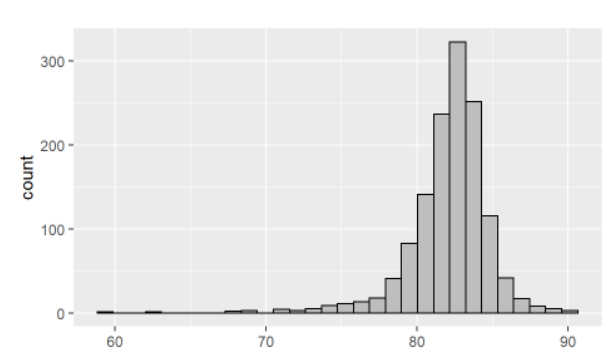
\includegraphics[width=4in]{images/hist1.png} \\
    {\small\textit{An example of a histogram with $n=30$ bins}}
\end{center}
Histograms can be used to determine the shape of a numerical variable distribution. If most of the data is to the right, as is the case in the figure above, then we say that the distribution is \textit{left-skewed}. Conversely, if most of the data is to the left, then we say that the distribution is \textit{right-skewed}. If the data is centered, then we say it is \textit{symmetric}.
\spacer
Another way to characterize the data is by its \textit{modality} or number of ``peaks'' in a distribution. The figure above represents a \textit{unimodal} distribution, since it shows one clear ``peak''. The following diagram shows other descriptions of modality with a corresponding example histogram.
\begin{center}
    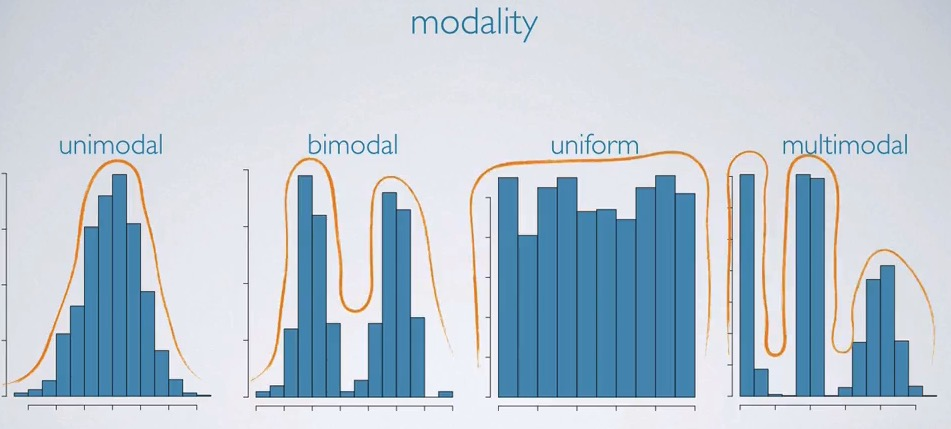
\includegraphics[width=5in]{images/modality.jpg}
\end{center}
Here is a useful diagram showing the relative positions of various common statistical measures in a histogram:
\begin{center}
    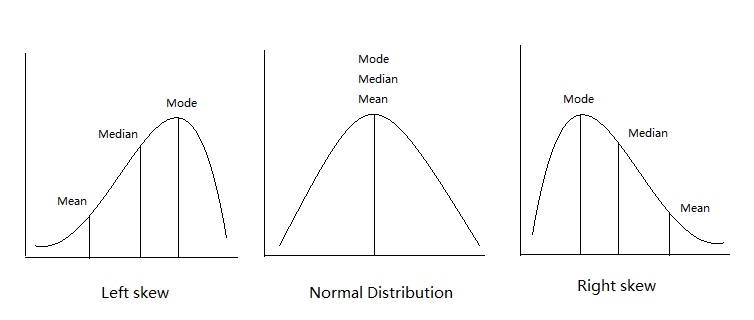
\includegraphics[width=5in]{images/hist2.png}
\end{center}
\subsubsection{Histograms in R}
The code to produce a histogram with 30 bins is as follows:
\begin{rcode}
ggplot(data=DATA, aes(x=VARIABLE)) + 
    geom_histogram(
        color="black",
        fill="gray",
        bins=30
    ) +
    labs(x="X-AXIS LABEL")
\end{rcode}
where \texttt{DATA} is some tibble, and \texttt{VARIABLE} is the variable being plotted. 
\subsubsection{Boxplots}
A boxplot is a way of visualizing some specific features of a numerical distribution, including spread and center. A boxplot is usually constructed using five values:
\begin{itemize}
    \item $Q_2$: the \textbf{median} or 50th percentile
    \item $Q_1$: the 25th percentile
    \item $Q_3$: the 7th percentile
    \item IQR: the \textit{inter-quartile range}, computed as $Q_3-Q_1$
    \item $1.5\cdot \text{IQR}$: the standard threshold for determining \textit{outliers}
\end{itemize}
Here you can see an example of a boxplot:
\begin{center}
    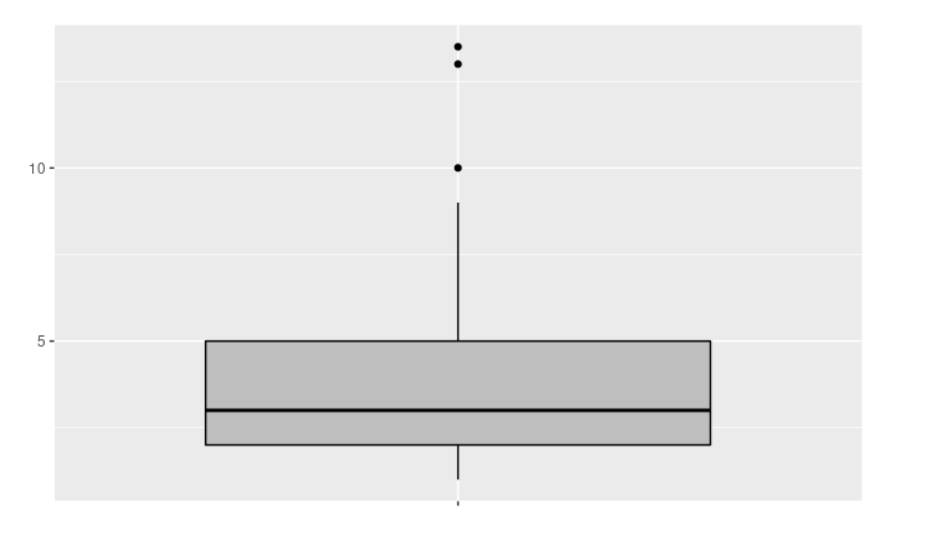
\includegraphics[width=4in]{images/bp1.png}
\end{center}
First consider the grey box. The top of the box is placed at $Q_3$, the line in the middle is the median, $Q_2$, and the bottom of the box is $Q_1$. The height of the box is therefore the IQR. Then, two whiskers are drawn above and below the boxes to a distance of 1.5 times the IQR. The bottom takes the lowest value in the distribution within this range, and similarly, the upper whisker takes the largest value in the distribution with this range. Values outside the range of the whiskers are called \textit{outliers} and are represented with a dot. Specifically, the end of the bottom whisker is placed at
$$
    \min \{x\in X:x\geq Q_1-1.5(Q_3-Q_1)\}
$$
and the end of the top whisker at
$$
    \max \{x\in X:x\leq Q_3+1.5(Q_3-Q_1)\}
$$
where $X$ is the set of variable observations used to construct the boxplot.
\spacer
If the data is skewed, the position and size of the box in a boxplot will represent that. If the size of the box is fairly small relative to the range of the data, it may be reasonable to conclude that the data is also unimodal.
\subsubsection{Boxplots in R}
\begin{rcode}
ggplot(data=DATA, aes(x=CATEGORY, y=VARIABLE)) + 
    geom_histogram(
        color="black",
        fill="gray"
    ) +
    labs(
        x="X-AXIS LABEL",
        y="Y-AXIS LABEL"
    )
\end{rcode}
The code to render a boxplot is similar to that used for histograms. In this case, \texttt{CATEGORY} is the name of a categorical variable to split the plots by category. If only one plot is desired, use \texttt{x=""}, where an empty string is used in place of \texttt{CATEGORY}. For instance, consider a tibble with rows of numerical variable \texttt{x} and categorical variable $\texttt{color}\in\{\texttt{RED}, \texttt{BLUE}\}$. If we wanted to create a boxplot with all values of \texttt{x}, we would use \texttt{aes(x="", ...)}. If we wanted to create two separate boxplots, one with values of \texttt{x} with the category ``RED'', and another to the side with values of \texttt{x} with the category ``BLUE'', we would use \texttt{\texttt{aes(x=color, ...)}}
\subsubsection{Barplots}
Barplots are visualizations of categorical data. A bar plot presents a bar for each possible category, with the length of each bar proportional to the number of observations of that category.
\todo
\section{Module 3 - Tidy Data}
\subsection{What is Tidy Data?}
\subsubsection{Definition}
Tidy data is characterized by data that is ``easy'' to understand by computers. ``Un-tidy'' data can be recognized by its difficulty to use in code without prior manipulation. Here is a more precise definition:
\begin{definition}[Tidy data]
    \textbf{Tidy data} is characterized by three rules:
    \begin{enumerate}
        \item Each variable must have its own column.
        \item Each observation must have its own row.
        \item Each value must have its own cell.
    \end{enumerate}
\end{definition}
In R, cells are allowed to be ``empty'' (i.e. having a value of \texttt{NA}). Even if data contains missing or \texttt{NA} values, it may still be considered tidy.
\subsubsection{Examples}
Consider the following data:
\spacer
\begin{center}
    \begin{tabular}{|l|l|l|l|}
\hline
\rowcolor[HTML]{EFEFEF} 
\textbf{Student} & \textbf{HW1} & \textbf{HW2} & \textbf{HW3} \\ \hline
Bob              & 75           & 93           & 88           \\ \hline
Alice            & 55           & 87           & 78           \\ \hline
Sarah            & 66           & 91           & 87           \\ \hline
\end{tabular}
\end{center}
Although this data appears neat (i.e. it is easily understood and well organized), it is not considered tidy. The rule that is violated here is \textbf{2. Each observation must have its own row}. If we consider a student's grade on some assignment to be a variable, it becomes apparent that we have three observations of this variable per row. Instead, to make this data ``tidy'', we would want it formatted like so:
\begin{center}
    \begin{tabular}{|l|l|l|}
\hline
\rowcolor[HTML]{EFEFEF} 
\textbf{Student} & \textbf{Grade} & \textbf{Assignment Number} \\ \hline
Bob              & 75             & 1                          \\ \hline
Bob              & 93             & 2                          \\ \hline
Bob              & 88             & 3                          \\ \hline
...              & ...            & ...                        \\ \hline
\end{tabular}
\end{center}
\subsection{Data Wrangling}
Data wrangling is the practice of transforming data to make it more useful. Some examples of data wrangling include:
\begin{itemize}
    \item Making data \textit{tidy}
    \item Adding or removing variables/columns
    \item Removing missing observations
\end{itemize}
\subsubsection{Data Wrangling Functions - \texttt{filter()}}
\begin{rcode}
data %>% filter(CONDITION)
\end{rcode}
The above expression returns a copy of \texttt{data}, including only rows for which the boolean expression \texttt{CONDITION} is true. Remember that in R, \texttt{\&} refers to logical AND rather than the conventional \texttt{\&\&}, and \texttt{|} refers to logical OR rather than the conventional \texttt{||}.
\spacer
For instance, given the tibble \texttt{grades} (represented below)
\begin{center}
    \begin{tabular}{|l|l|l|}
\hline
\rowcolor[HTML]{EFEFEF} 
\texttt{student} & \texttt{grade} & \texttt{assn\_no} \\ \hline
Bob              & 75             & 1                          \\ \hline
Bob              & 93             & 2                          \\ \hline
Bob              & 88             & 3                          \\ \hline
...              & ...            & ...                        \\ \hline
\end{tabular}
\end{center}
the code
\begin{rcode}
grades <- grades %>% filter(grade > 80) 
\end{rcode}
would remove all instances of grades below 80\%.
\spacer
The \texttt{is.na()} function can also be used in conjunction with \texttt{filter} to remove or extract missing (\texttt{NA}) values.
\subsubsection{Data Wrangling Functions - \texttt{select()}}
\begin{rcode}
data %>% select(VAR1, VAR2, VAR3, ...)
\end{rcode}
\texttt{select} takes the passed dataframe and a list of variables/columns, and returns a copy with only those variables/columns.
\subsubsection{Data Wrangling Functions - \texttt{mutate()}}
\begin{rcode}
data %>% mutate(NEW_VARIABLE=VALUE)
data %>% mutate(NEW_VARIABLE=case_when(
    CONDITION1 ~ VALUE1,
    CONDITION2 ~ VALUE2,
    ...
))
\end{rcode}
\todo
\subsubsection{Data Wrangling Functions - \texttt{arrange()}}
\begin{rcode}
data %>% arrange(VAR)       # sort by ascending
data %>% arrange(desc(VAR)) # sort by descending
\end{rcode}
\texttt{arrange} returns a sorted copy of a dataframe, sorted by a given variable.
\subsubsection{Summary Tables in R}
A summary table is an easy way to view certain statistics about a dataframe. Consider the tibble \texttt{data} representing the following data:
\spacer
\begin{center}
    \begin{tabular}{|l|l|}
\hline
\rowcolor[HTML]{EFEFEF} 
\textbf{\texttt{name}} & \textbf{\texttt{age}} \\ \hline
Jerry                  & 24                    \\ \hline
Alex                   & 31                    \\ \hline
Winston                & 40                    \\ \hline
\end{tabular}
\end{center}
The code
\begin{rcode}
data %>% summarize(
    n=n(),
    mean_age=mean(age),
    median_age=median(age),
)
\end{rcode}
Produces the following tibble:
\begin{center}
    \begin{tabular}{|l|l|l|}
\hline
\rowcolor[HTML]{EFEFEF} 
\textbf{\texttt{n}} & \textbf{\texttt{mean\_age}} & \texttt{median\_age} \\ \hline
3                   & 31.667                     & 31                  \\ \hline
\end{tabular}
\end{center}
Below are a list of functions that can be used in a summary table:
\spacer
\begin{tabular}{|l|l|}
\hline
\rowcolor[HTML]{EFEFEF} 
\textbf{Function} & \textbf{Description}                      \\ \hline
\texttt{n()}      & Returns the number of observations        \\ \hline
\texttt{mean()}   & Returns the mean                          \\ \hline
\texttt{min()}    & Returns the minimum                       \\ \hline
\texttt{max()}    & Returns the maximum                       \\ \hline
\texttt{median()} & Returns the median                        \\ \hline
\texttt{var()}    & Returns the variance ($\sigma^2$)         \\ \hline
\texttt{sd()}     & Returns the standard deviation ($\sigma$) \\ \hline
\texttt{sum()}    & Returns the sum                           \\ \hline
\end{tabular}
\spacer
Using the function \texttt{group\_by} first will separate the statistics by the name of the passed categorical variable.
\section{Module 4 - One Proportion Hypothesis Testing}
\subsection{Introduction to Statistical Inference}
\begin{definition}
    \textbf{Statistical inference} is the process of coming to conclusions or decisions based on statistical information.
\end{definition}
Conclusions made using statistical information are subject to uncertainty; in statistical inference, nothing should be stated as fact.
\spacer
Statistical inference often uses techniques involving \textit{sampling}; taking a small subset of the potentially available information and analyzing that. The following terms are often used in this context:
\begin{itemize}
    \item \textbf{Population}: A complete set of items, events, or data that is of interest for statistical inference.
    \begin{itemize}
        \item The population can be thought of as ``the entire thing we are trying to study''.
        \item The population may be too large to feasibly observe, or may be hypothetical or infinite in size.
        \item The goal of statistical inference is to devise some conclusion about the population without having to observe the entire population.
    \end{itemize}
    \item \textbf{(Population) Parameter}: In statistical inference, the parameter is some ``true'' measure of the population that is trying to be inferred.
    \begin{itemize}
        \item Sometimes written as $p$ or $\pi$
    \end{itemize}
    \item \textbf{Sample}: Refers to a manageable subset of the population that can be reasonably observed.
    \begin{itemize}
        \item A good sample is one that is \textit{representative} of the population; oftentimes, it is best to choose a random sample.
    \end{itemize}
    \item \textbf{Test Statistic}: A quantity or measure derived from the sample that can be used to estimate the parameter.
    \begin{itemize}
        \item Often denoted $\hat p$ or $\hat \pi$.
    \end{itemize}
    \item \textbf{Sampling Distribution}: A probability distribution of test statistics for all possible samples of the same sample size.
    \begin{itemize}
        \item Often represented in a histogram.
    \end{itemize}
\end{itemize}
Here are some common symbols used for various statistical measures used in hypothesis testing:
\begin{center}
    \begin{tabular}{|l|l|l|}
\hline
\rowcolor[HTML]{EFEFEF} 
\textbf{Statistic Type} & \textbf{Population} & \textbf{Sample} \\ \hline
Proportion              & $p$                 & $\hat p$        \\ \hline
Mean                    & $\mu$               & $\bar x$        \\ \hline
Median                  & (no common symbol)  & $\tilde x$      \\ \hline
\end{tabular}
\end{center}
\newpage
\subsubsection{Hypothesis Testing}
Hypothesis testing is a form of statistical inference, and involves coming up with a hypothesis and trying to prove that it is incorrect. Hypothesis testing generally takes the following steps:
\begin{enumerate}
    \item Devise a \textit{null hypothesis} and an \textit{alternative hypothesis}.
    \begin{enumerate}
        \item The null hypothesis:
            \begin{definition}
                The \textbf{null hypothesis} is a conjecture that a hypothesis test will try to disprove. In general, the null hypothesis represents the ``default'' outcome in statistical inference, usually something along the lines of ``no effect'' or ``no difference''.\spacer
                In a court of law, the null hypothesis is ``innocent'' under the philosophy of ``innocent until proven guilty''.
            \end{definition}
        \item The alternative hypothesis:
            \begin{definition}
                The \textbf{alternative hypothesis} is a statement that exists as the ``alternative'' option to the null hypothesis. The null hypothesis and the alternative hypothesis must be mutually exclusive, and in general, the alternative hypothesis is simply the opposite of the null hypothesis.
            \end{definition}
        \item The null hypothesis is often written $H_0$, and the alternative hypothesis is written as $H_1$ or $H_A$. When stating the hypothesis, we write
        $$
            H_0:P\quad\text{and}\quad H_A: Q
        $$
        where $P$ and $Q$ are some statements representing the null and alternative hypotheses respectively. Because the null hypothesis is a label, not a variable, we use a colon.
    \end{enumerate}
    \item Create a sample and compute a test statistic based on the sample.
    \item Estimate a sampling distribution, usually by simulation. We assume the null hypothesis is true.
    \item Calculate a $p$-value to quantify evidence against the null hypothesis.
        \begin{definition}
            A \textbf{$p$-value} is defined as the probability of obtaining a result at least as extreme as the test statistic. 
        \end{definition}
    \item Draw a conclusion based on the $p$-value. For this, the following guideline is conventionally used:
    \begin{center}
        \begin{tabular}{|l|l|}
\hline
\rowcolor[HTML]{EFEFEF} 
\textbf{$p$-value} & \textbf{Evidence}                  \\ \hline
$p>0.10$           & No evidence against $H_0$          \\ \hline
$0.05<p<0.10$      & Weak evidence against $H_0$        \\ \hline
$0.01<p<0.05$      & Moderate evidence against $H_0$    \\ \hline
$0.001<p<0.01$     & Strong evidence against $H_0$      \\ \hline
$p<0.001$          & Very strong evidence against $H_0$ \\ \hline
\end{tabular}
    \end{center}
\end{enumerate}
\begin{aside}
    \textbf{Statistical Significance}
    \spacer
    In general, we have some value $\alpha$, under which if $p<\alpha$, then the null hypothesis is false. Conventionally, we use $\alpha=0.05$. If this is the case, that is, $p<\alpha$, then the findings are said to be \textit{statistically significant}.
\end{aside}
\subsubsection{Example}
One common example for statistical inference is measuring the ``fairness'' of a coin. Consider a coin that can land on either heads or tails, and we want to answer the question of ``is this coin equally likely to land on heads as it is tails, that is, is this coin \textit{fair}?
\spacer
For this, we say that the \textit{population} is the outcomes of the set of all possible coin flips. Then, our parameter $p$ is the proportion of those coin flips that land on heads.  As we can see, our population is theoretically infinite, and therefore infeasible to measure directly; however, we can loosely define our parameter using the following expression\footnote{We use limit notation in this case, as using $\infty$ directly in our expression for $p$ would look strange.}
$$
    p=\lim_{n\to\infty}\left(\frac{1}{n}\sum_{i=1}^n F_i\right)
$$
Where, if the coin were to be flipped an arbitrarily large number of times, $F_n$ would be the result of the $n$th coin flip, 1 if heads, and 0 if tails.
\spacer
Let us continue by defining our hypotheses. As stated earlier, the null hypothesis is often similar to the phrase ``no difference''. Therefore, we will assume that there is no difference between the probability of the coin landing on heads and the coin landing on tails. Therefore, we define our hypotheses as follows:
$$
    H_0:p=0.5\quad\text{and}\quad H_A:p\neq 0.5
$$
\spacer
Given that our population is infinite, we need to define a finite sample of the population on which to perform inference. Let $n$ be our sample size, which may be chosen arbitrarily. For this example, we will use $n=50$. Then, we can compute the test statistic as
$$
    \hat p= \frac{1}{50}\sum_{i=1}^{50}F_i
$$
Where in this case $F_n$ is the observed $n$th result of actually flipping the coin. For this example, we will pretend that $\hat p=0.56$, that is, 28 out of 50 coin flips were heads.
\spacer
To estimate a sampling distribution to find out where our test statistic falls, we will assume that the null hypothesis is true, that is, $p=0.5$, and simulate a distribution of test statistics for samples also of size $n=50$. This can be done using the \textit{binomial distribution function}, but for simplicity, we can also use a computer program to flip an imaginary coin many times. Remember that the $p$-value is defined as the probability that we observe a result in our sampling distribution as or more extreme than our test statistic. We define ``as or more extreme'' in this case as being the same distance or farther away from 0.5 than the test statistic. Therefore, our $p$-value is the proportion of values in our sampling distribution that are as or more extreme than $\hat p$. Let $s_1,s_2,\dots,s_N$ be the results of our our simulated sampling distribution where $s_n$ is the proportion of a simulated fair coin landing on heads, where the coin is flipped 50 times, just like in our sample. To make our sampling distribution as accurate as possible, we will make $N$ very large, say, $N=100\,000$.
$$
    \text{$p$-value}=\frac{1}{N}\sum_{i=1}^N \begin{cases}1&|s_i-0.5|\geq|\hat p - 0.5|\\0&\text{otherwise}\end{cases}
$$
Using a computer program to fill in values for $s_i$, we find a $p$-value of about $0.40$. By the table in the previous section, we see that we have no evidence against our null hypothesis that our coin is fair, and therefore our \textit{conclusion} is that the coin is, in fact fair.
\section{Module 5 - Randomization Testing}
\subsection{Motivating Example - Two Group Hypothesis Testing}
Consider an experimental drug that is designed to lower blood pressure. We have two groups, a \textit{treatment} group, which receives this drug, and a \textit{control} group which does not (or receives a placebo, etc.). The population in this case, would be a hypothetical infinite set of patients in each group, and we want to find whether the \textit{mean} blood pressure is lower in the group that received the treatment. Hence, we call our parameters $\mu_{treatment}$ and $\mu_{control}$ respectively.
\spacer
Our null hypothesis is that the drug has \textit{no effect}, that is, $\mu_{treatment}=\mu_{control}$. We then label our hypotheses
$$
    H_0:\mu_{treatment}=\mu_{control}\quad\text{and}\quad H_A:\mu_{treatment}\neq \mu_{control}
$$
or alternatively,
$$
    H_0:\mu_{treatment}-\mu_{control}=0\quad\text{and}\quad H_A:\mu_{treatment}- \mu_{control}\neq 0
$$
Say we then derive a \textit{sample} of 50 patients for both the treatment and control group, running the experiment accordingly. We then have values for our \textit{test statistic}, $\bar x$, the mean blood pressures of each sample group. Say we find that\footnote{Using arbitrary units for blood pressure}
$$
    \bar x_{treatment} = 92.1\quad\text{and}\quad\bar x_{control}=103.4
$$
Hence,
$$
    \bar x =\bar x_{treatment}-\bar x_{control} = -11.3
$$
How do we derive a $p$-value to measure the likelihood that our null hypothesis is false, that is, how do we know whether the drug was effective?
\subsection{Randomization Testing}
Continuing with the earlier example involving a hypothetical drug trial, we need a method to simulate a sampling distribution under the null hypothesis to see whether or not our test statistic was ``likely'' or not. Under the null hypothesis, we assume that there is no difference between the treatment and control groups. Therefore, given some observation for a blood pressure measure, we could say that under the null hypothesis, it is equally likely that measure belonged to the control group or the treatment group.
\spacer
Hence, one way to simulate a sampling distribution is to take the all the blood pressure measures of the treatment group and all blood pressure measures into the control group and combine them into a series of observations $x_1,x_2,\dots x_n$. We then take the ``labels'' of each observation, either ``Control'' or ``Treatment'' (in our example there is an equal number of both), and combine them into a series of labels $L_1,L_2,\dots,L_n$ as well. We then shuffle the labels and observations around independently, and construct a set of tuples $(x_i,L_i)$ that effectively rematches each label to a random observation.
\spacer
We may then compute a test statistic $\bar x$ for our sampling distribution based on our simulated sample as so:
$$
    \begin{aligned}
    \bar x &= \text{mean treatment} - \text{mean control} \\
    &= \frac{\sum \text{treatment observations}}{\#\,\text{treatment}} - \frac{\sum \text{control observations}}{\#\,\text{control}}
    \end{aligned}
$$
Specifically,
$$
    \bar x =  \frac{\displaystyle \sum_{i=1}^n x_i\cdot\left(\begin{cases}1&L_i=\text{``Treatment''} \\ 0&\text{otherwise}\end{cases}\right)}{\displaystyle \sum_{i=1}^n\begin{cases}1&L_i=\text{``Treatment''} \\ 0&\text{otherwise}\end{cases}} -   \frac{\displaystyle \sum_{i=1}^n x_i\cdot\left(\begin{cases}1&L_i=\text{``Control''} \\ 0&\text{otherwise}\end{cases}\right)}{\displaystyle \sum_{i=1}^n\begin{cases}1&L_i=\text{``Control''} \\ 0&\text{otherwise}\end{cases}}
$$
Repeating the shuffling and recomputation of $\bar x$ an arbitrary number of times produces a sampling distribution, from which a $p$-value can be calculated as the proportion of simulated $\bar x$ that are farther away from 0 than our test statistic.
\subsection{Type I and Type II Errors}
Hypothesis testing is imperfect by nature. Sometimes, it is possible to arrive at the wrong conclusions.
\subsubsection{Type I Error}
A type 1 error, sometimes referred to as a \textit{false positive}, refers to the incorrect rejection of a null hypothesis, that is, we conclude that the null hypothesis is false, when it is actually true. Some examples include:
\begin{itemize}
    \item A COVID-19 test returning positive, when the user was not infected.
    \item An innocent person being convicted.
\end{itemize}
In a hypothesis test, this is often because the observed test statistic was just very unusual.
\subsubsection{Type II Error}
A type 2 error, sometimes referred to as a \textit{false negative}, refers to the mistaken acceptance of a null hypothesis, that is, we conclude that the null hypothesis is true, when it is actually false. Some examples include:
\begin{itemize}
    \item A COVID-19 test returning negative, when the user is actually infected.
    \item A medical screening fails to refer someone to a physician for further testing.
    \item An guilty person being deemed innocent.
\end{itemize}
\section{Module 6 - Bootstrap and Confidence Intervals}
\subsection{Introduction to Estimation}
\subsubsection{Motivation}
There are a few problems with $p$-value based hypothesis testing:
\begin{enumerate}
    \item Scientific studies are often too reliant on $p$-values; it is possible to intentionally misuse $p$-values to make misleading arguments.\footnote{This is sometimes called \textit{$p$-hacking}.}
    \item The choice of $\alpha=0.05$ as the threshold for statistical significance, while conventional, is still arbitrary.
    \item Hypothesis testing can only tell us if something is true or not; it doesn't give us any more information than that.
\end{enumerate}
\begin{aside}
    \textbf{Types of Sampling}
    \spacer
    Moving forward, it is worth differentiating the notions of \textit{sampling with replacement} and \textit{sampling without replacement}. The typical idea of ``taking a sample of size $n$ from a population'' does not usually involve replacement. Specifically, when we sample without replacement, the same member of the population cannot be sampled twice.
\spacer
Sampling \textit{with replacement}, on the other hand, can be thought of using an analogy of a bag of colored marbles. When we take a sample of size $n$ with replacement, we take a marble from the bag, record its color, put the marble back in the bag (\textit{replace} it), and repeat $n$ times. If we were to sample \textit{without replacement}, we would not put each marble back after taking it out.
\end{aside}
\subsubsection{What is Estimation?}
Confidence interval estimation involves using a sample to make a reasonable guess about the value of some population parameter, and placing an interval around that guess to represent a conclusion about the rest of the population.
\spacer
Estimation, like hypothesis testing, uses notions of populations, samples, parameters, test statistics, and sampling distributions. Imagine a population such as the heights of every male adult on Earth, and we want to find the population mean, that is, the average male height. We take a random sample of 100 men, and say that we find the average height of this sample to be about 5'8'' (173 cm). Unlike hypothesis testing, there is no ``null hypothesis'' under which to sample, so what would a sampling distribution for this statistic look like, and how would we find one?  The most theoretically straightforward answer would be to simply take more random samples from the population of the same size (100 men).
\begin{aside}
    \textbf{Sampling Distributions and Sample Size}
    \spacer
    How would the sample size affect the shape of a sampling distribution of means? Consider two extremes of sample size $n$, one where $n$ is the size of the population itself, and another where $n=1$. If we were to sample without replacement samples the size of the entire population, each sample mean would simply be the population mean. A histogram for that distribution would have a single value, a distinct mode, and be perfectly symmetrical.
    \begin{center}
        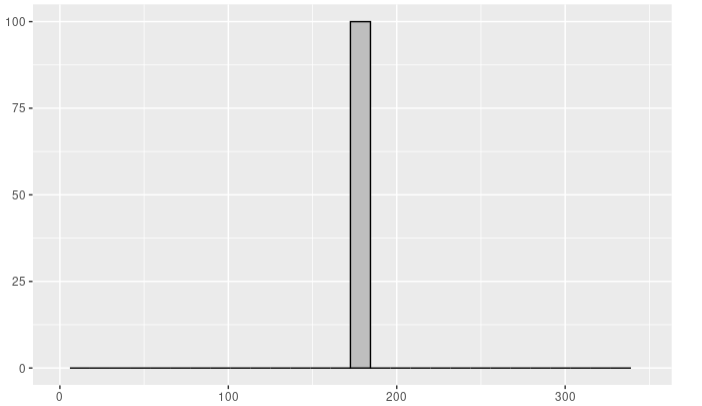
\includegraphics[width=3in]{images/hist3.png}
    \end{center}
    Conversely, a sampling distribution of $n=1$ would look very similar to the distribution of the data itself. It may be skewed, multimodal, etc. In general, as the sample size $n$ increases:
    \begin{enumerate}
        \item The mean of the sampling distribution stays roughly the same and approximates the population mean.
        \item The shape of the sampling distribution becomes less skewed.
        \item The spread of the sampling distribution decreases.
    \end{enumerate}
\end{aside}
If we were to repeatedly take more random samples from the population, we would get a very good representation of a sampling distribution. However, in the example where our population is the heights of every man on Earth, it is feasible to keep taking random samples from the population, otherwise we would survey the entire population itself. 
\spacer
The only way to create a sampling distribution, then, is to estimate one from the one sample itself.
\subsection{Bootstrap Sampling}
Bootstrap sampling is the process of estimating a sampling distribution from a single sample. If we assume that the sample taken is representative of the population (which should be the case if it was randomly sampled), then we can create a sampling distribution from the sample, by repeatedly \textit{sampling the sample with replacement}. If we sampled without replacement, then the sampling distribution would be perfectly homogeneous; however, sampling with replacement allows some variability in our sampling distribution that emulates the variability in the population sampling distribution.
\spacer
Although this method seems like it would not work--after all it seems to create new data out of thin air--it proves to be a useful method in estimating a sampling distribution, so long as the original sample is representative of the population.
\subsection{Confidence Intervals}
So far, we have been able to use bootstrap sampling to create a sampling distribution, but the question of how to use these methods to create an estimation of a population parameter still remains. For this, we use a measure called a confidence interval.
\subsubsection{Definition}
A 95\% \textbf{confidence interval} for a population parameter is defined as some interval such that, for 95\% of possible random samples from the population, that interval will contain the true parameter. Specifically, say we compute a bootstrap sampling distribution, represented using the variable $x$ with observations $x_1,x_2,\dots x_n$, where each $x_i$ is the mean of some bootstrapped sample from our original ``true'' sample. 
\begin{aside}
    In this context, 95\% is called the \textbf{confidence level}, and is by far the most commonly used value, but other values such as 90\% and 99\% are also sometimes used. Specifically, for some a confidence level $c\in[0,1]$, if we were to take many random samples from the population, computing a bootstrap confidence interval (with confidence level $c$) for each one, $c$ represents the proportion of those confidence intervals that contain the actual parameter.
\end{aside}
Recall that for some $p\in[0,100]$, the $p$th percentile of some variable is the smallest value such that $p\%$ of those of the observations of that variable are less than $p$. Thus, a 95\% confidence interval $[a,b]$ is defined where $a$ is the 2.5th percentile, and $b$ is the 97.5th percentile.
\begin{aside}
     Notice that the range of values between $a$ and $b$ covers 95\% of the observed values. If we were to more intuitively pick $a$ and $b$ to be the 5th and 95th percentiles respectively, we would end up with a 90\% confidence interval instead.
\end{aside}
\subsubsection{Interpreting Confidence Intervals}
Say we concluded a 95\% confidence interval of $[165.3, 182.1]$ (measured in centimeters) for our earlier sample of 100 men's heights. What we say from this information is that we are ``95\% confident that the mean adult male height globally is between 165.3 and 182.1 centimeters''. Note that we don't say that there is a ``95\% chance'', only that we are ``95\% confident''.

\section{Module 7 - Simple Linear Regression}
\subsection{Association of Numerical Variables}
\textbf{Association} between two numerical variables refers to variables that can be related mathematically. A common way that variables can be associated is using a scatterplot, a diagram used to show correlation between observations of two variables $x$ and $y$, by representing them as a set of points $(x_i, y_i)$ on the Cartesian plane for each $i$th observation.
\subsubsection{Features of Association}
\begin{itemize}
    \item \textbf{Form}: describes the pattern that two variables follow together (e.g. linear, non-linear, quadratic, etc.)
    \begin{itemize}
        \item These labels are not mutually exclusive; if a pattern is quadratic, it is also non-linear by definition.
    \end{itemize}
    \item \textbf{Direction}: describes an overall overall trend.
    \begin{itemize}
        \item Two variables are said to be \textbf{positively associated} if values of one variable increase as the other increases.
        \item Two variables are said to be \textbf{negatively associated} if values of one variable decrease as the other decreases.
    \end{itemize}
    \item \textbf{Strength}: describes how concentrated the values of the variable are around the pattern.
\end{itemize}
\subsubsection{Scatterplots in R}
\begin{rcode}
heights %>% ggplot(aes(x=X_VARIABLE, y=Y_VARIABLE, color=CATEGORY))
		+ geom_point()
		+ labs(x="X AXIS LABEL", y="Y AXIS LABEL"))
		+ theme_minimal() # optional
\end{rcode}
The \texttt{color} argument is optional, and can be used to color-code the points based on the value of some categorical variable. Alternatively, adding \texttt{facet\_wrap(\~CATEGORY)} will split the data into two scatterplots. As an example, here is the output produced by the following code, where \texttt{heights} is a data frame where each row contains information about a person's height, sex, and shoe print length.
\begin{rcode}
heights %>% ggplot(aes(x=shoePrint, y=height))
		+ geom_point()
		+ labs(x="Length of shoeprint (in cm)", y="Height (in cm)"))
		+ theme_minimal()
		+ facet_wrap(~sex)
\end{rcode}
\begin{center}
    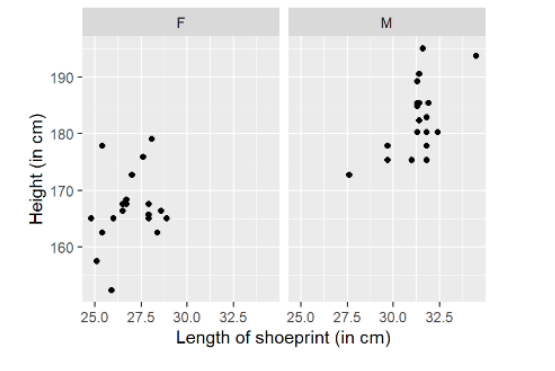
\includegraphics[width=4in]{images/scatter1.png}
\end{center}
\subsubsection{Quantifying Linear Association - Correlation}
\textbf{Correlation} is a value, written $r$, between -1 and 1, that summarizes the strength and direction of the linear relationship between two numerical variables.
\spacer
Given a set of data points $(x_1,y_1),(x_2,y_2),\dots,(x_n,y_n)$ for a set of variable observations, the mean value for $x$, $\bar x$, and the mean value for $y$, $\bar y$, $r$ is given as
$$
    r=\frac{\displaystyle \sum_{i=1}^n(x_i-\overline x)(y_i-\overline y)}{\displaystyle \sum_{i=1}^n (x_i-\overline x)^2\cdot\sum_{i=1}^n (y_i-\overline y)^2}
$$
The correlation value has the following properties that describe the strength and direction of the linear association:
\begin{itemize}
    \item $r>0$ denotes a positive linear association.
    \item $r<0$ denotes a negative linear association
    \item $r=0$ denotes a perfectly flat linear association or no correlation at all.
    \item The higher the magnitude of $r$, $|r|$, the stronger the linear association.
\end{itemize}
The following code can be used to compute $r$ in R.
\begin{rcode}
corr(
	x=heights$shoePrint,
	y=heights$height
)
\end{rcode}
\begin{aside}
     Remember that $r$ only quantifies the \textit{linear} association between two variables. Even if they are associated perfectly in another way, say quadratically, they may have a very low $r$ value.
\end{aside}
\subsection{Simple Linear Regression}
The \textbf{simple linear regression model} assumes a ``best'' straight line that summarizes the real relationship between two variables $x$ and $y$, and that the values only deviate from this line. The model can be summarized using the following equation:
$$
    Y_i=\beta_0+\beta_1x_i+\varepsilon_i
$$
Where
\begin{itemize}
    \item $Y_i$: The response variable (or dependent variable, target variable, etc.) for observation $i$.
    \item $x_i$: The independent variable (or predictor, covariate, feature, input, etc.) for observation $i$.
    \item $\beta_0$: The intercept parameter.
    \item $\beta_1$: The slope parameter.
    \item $\varepsilon_i$: A random error term for observation $i$ that accounts for deviation from the line defined by $y=\beta_1x+\beta_0$.
\end{itemize}
\subsection{Fitting a Regression Line}
Recall that the simple linear regression model assumes the existence of some line described by the equation
$$
    Y_i=\beta_0+\beta_1x_i
$$
(and an extra error term $\varepsilon_i$ to account for deviations). But this does not tell us what the values of $\beta_0$ and $\beta_1$ are. There is no way to determine the ``true'' values of these parameters. But we can use various mathematical models to find best estimates for these values, denoted $\hat \beta_0$. and $\hat \beta_1$.
\begin{aside}
    In the context of linear regression, and often other statistical models, a carat or ``hat'' above a variable often denotes that this variable is an \textit{estimate} or a \textit{prediction}.
\end{aside}
\subsubsection{Least Squares Regression Line}
The least squares regression method finds values for $\hat \beta_0$ and $\hat \beta_1$ that \textit{minimize} the squared error between $\hat y$, the predicted values for $y$, and the true values of $y$, where
$$
    \hat y = \hat \beta_0 + \hat \beta_1 x
$$
This method produces the following closed-form mathematical expressions for the estimated values of $\beta_0$ and $\beta_1$:
$$
    \hat \beta_0=\bar y - \hat \beta_1 \bar x
$$
and
$$
    \hat \beta_1 = \frac{\displaystyle\sum_{i=1}^n(x_i-\bar x)(y_i-\bar y)}{\displaystyle\sum_{i=1}^n (x_i-\bar x)^2}
$$
where $\bar x$ and $\bar y$ are the sample means of the $x$ and $y$ observations respectively.
\subsubsection{Interpretation of Regression Coefficients}
The estimated values found above produce a way to predict new values for $y$, given some value for $x$, using the following equation:
$$
    \hat y = \hat \beta_0 + \hat \beta_1 x
$$
$\hat y$ is called the \textbf{fitted value} or \textbf{predicted value} and is the estimated value for $y$ when the predictor takes a value of $x$. The equation above is called the \textbf{fitted regression line} and its slope is given by $\hat \beta_1$, and its $y$-intercept by $\hat \beta_0$. The difference between the observed and predicted value of $y$ for the $i$th observation is called the \textbf{residual} $e_i=y_i-\hat y_i$.
\subsubsection{Coefficient of Determination}
The \textbf{coefficient of determination}, written $R^2$, is a number between 0 and 1 that measures the proportion of variability in $y$ that is explained by a fitted regression line.
$$
    R^2=1-\frac{\displaystyle\sum_{i=0}^n (y_i-\hat y_i)^2}{\displaystyle\sum_{i=0}^n (y_i-\overline y)^2}=r^2
$$
\begin{itemize}
    \item A value of $R^2$ close to 1 indicates that most of the variability in $y$ is explained by the regression model.
    \item A value of $R^2$ close to 0 indicates that very little of the variability in $y$ is explained by the regression model.
    \item $R^2$ is also equal to $r^2$, where $r$ is the correlation value.
\end{itemize}
\subsection{Linear Regression with Categorical Variables}
If we wanted to have the independent variable $x$ be a binary categorical variable instead of a numerical one, we use an \textbf{indicator variable}. For this, we assign a \textbf{baseline value} to one category, the value corresponding to $x=0$, and assign $x=1$ to the other. \spacer
For instance, we may have
$$
    x_i=\begin{cases}1&\text{individual $i$ is male}\\0&\text{individual $i$ is female}\end{cases}
$$
where ``female'' is the baseline value.
\subsubsection{Interpreting $\hat \beta_0$ and $\hat \beta_1$}
Recall that 
$$
    \hat y = \hat \beta_0 + \hat \beta_1 x
$$
As an example, let $x$ be a categorical variable for sex as defined above, and let $\hat y$ be a prediction for height.
\spacer
Thus,
\begin{itemize}
    \item When $x=0$, (e.g. when our predictor is that some person is female), we have
    $$
        \hat y = \hat \beta_0 + \hat \beta_1 \cdot 0 = \hat \beta_0
    $$
    \item When $x=1$, (e.g. when our predictor is that some person is male), we have
    $$
        \hat y = \hat \beta_0 + \hat \beta_1 \cdot 0 = \hat \beta_0 + \hat \beta_1
    $$
\end{itemize}
Therefore, $\hat\beta_0$ is the predicted height for women (it is also the sample mean height for women), $\hat\beta_0+\hat\beta_1$ is the predicted height for men (it is also the sample mean height for men), and $\hat\beta_1$ is the average difference in height between men and women.
\section{Module 8 - Multiple Linear Regression}
\section{Module 9 - Classification}
\section{Module 10 - Ethics}
\end{document}
